\documentclass[a4paper]{article}
\usepackage[utf8]{inputenc}
\usepackage{multicol} % Allows for multiple columns
\usepackage{geometry} % Allows for custom page dimensions and margins
\usepackage{authblk} % Better handling of author affiliations
\usepackage{algorithm}
\usepackage{algpseudocode}
\usepackage{amsmath}
\usepackage{graphicx}
\usepackage{hyperref}
\usepackage[backend=biber, style=ieee]{biblatex}
\hypersetup{colorlinks=true}
\usepackage{amssymb}
\usepackage{amsthm}
\usepackage{booktabs}
\newtheorem{theorem}{Theorem}
\newtheorem{claim}{Claim}
\usepackage[flushleft]{threeparttable}
\usepackage[table]{xcolor}  % For coloring 
\definecolor{lightgray}{gray}{0.90}
\usepackage{changepage} % For changing the margins locally
\usepackage{gensymb}
\usepackage{subcaption}
\usepackage{float}
\usepackage[skip=2pt]{caption}

\addbibresource{BMED8803MLforNeuralData.bib}

% Setting reasonable page margins
\geometry{
  top=2.5cm,
  bottom=2.5cm,
  left=2.5cm,
  right=2.5cm
}

\title{\textbf{Predicting Entorhinal Grid Cell orientation from fMRI dataset using GLM and CNN}}

% Define authors with superscript numbers for affiliations
\author[1]{Sina Dabiri}
\author[2]{Rishi Dakarapu}
\author[3]{Danielle Dowe}

% Redefine the affiliation font and alignment
\renewcommand\Affilfont{\normalfont\small\raggedright} % Makes the affiliation text smaller and left aligned

% Define affiliations with proper email notations
\affil[1]{Department of Biomedical Engineering, Georgia Institute of Technology, Atlanta, Georgia}
\affil[2]{Department of Biomedical Engineering, Georgia Institute of Technology, Atlanta, Georgia}
\affil[3]{Department of Machine Learning, Georgia Institute of Technology, Atlanta, Georgia}

\date{} % This will remove the date

\begin{document}

\maketitle

% Section: Introduction
\section{Introduction}
\label{sec:introduction}

Spatial Navigation is one of the main cognitive functions of the human brain and entorhinal cortex’s (EC) gird cells plays an active role in navigation (\cite{hafting_microstructure_2005}, \cite{yartsev_grid_2011}). Researchers using fMRI have observed that the grid cell-like signal when subjects are navigating a virtual environment changes from the typical 6-fold preferred orientation when they are in an open field environment to a 4-fold preferred orientation when there are barriers in the environment (\cite{he_environmental_2019}). In addition, computational researchers have shown that Generalized Linear Model (GLM) are effective in estimating grid cell alignment and have developed a MATLAB toolbox for researchers (\cite{stangl_gridcat_2017}). In addition, previously computational researchers have shown that 3D convolutional neural nets (3D CNN) are able to extract spatial features with an accuracy of 69.15\% (\cite{zou_3d_2017}). Furthermore, in Dr. Brown’s lab at Georgia Tech, Adrian had shown that CNN is a promising method for real time estimation with low mean squared error (MSE) of 0.025. However, we later learned from him that he had data leak from training set into testing set and we need to redo the CNN modeling. 

 They tested 20 participants (9 females, ages 18-22) while they completed 12 runs of the virtual environment, 6 runs of open field (OF) and 6 runs of environments with hairpin barriers (BA). There were two types of indoor and outdoor environments, such that the indoor environments had patches of blue, yellow, black or green on east, south, west, and north walls and the outdoor environments had landmarks of tower, rock, tree, and cactus for the 4 directions. During navigation the subjects would reach waypoints marked by a red virtual arrow and they would answer spatial awareness questions such as, “Where is the green? Left or Right” for indoor environments and “Where is the cactus? Left or Right” for the outdoor environments. The birds eye view of the indoor and outdoor environments was the same.

There is a gap in the spatial navigation field in how to use CNN for real time alignment estimation of grid cell activity. This gap was addressed by first trying to implement a 3D CNN model. In addition, we implemented a 1D CNN model to measure alignments of grid cells. Lastly, we implemented a hybrid CNN-RNN (CNN-Long Short-Term Memory, CNN-LSTM) model to measure alignments.  

% Section: Methods
\section{Methods}
\label{sec:methods}

\noindent This study leverages advanced computational and neural modeling techniques to investigate grid cell-like activity in the human brain using fMRI data. We employed the GridCAT toolbox for initial modeling and visualization of grid cell symmetry (\cite{stangl_gridcat_2017-1} ), alongside novel machine learning architectures, including a 1D-CNN and a hybrid 1D-CNN-LSTM model, to analyze spatial and spatiotemporal patterns in voxel activation. GridCAT facilitated classical GLM-based analyses to quantify grid orientation coherence, while the custom-designed neural network models provided a robust framework for predicting continuous alignment scores, integrating spatial feature extraction with temporal dynamics. Comprehensive preprocessing pipelines were implemented to ensure data quality and consistency, including steps for signal normalization, temporal alignment, and feature scaling. This integrative approach allowed the study to capture intricate relationships between neural responses and behavioral paradigms, with a focus on enhancing interpretability and improving model performance. 


\subsection{Participants and Data Acquisition}
fMRI data from participants 5 and 14 were used to prototype the models. These subjects were selected for their reliable grid cell-like signals, as identified in preliminary analyses. Each subject completed 12 runs (six in an open-field environment and six in a barrier environment), with their virtual reality orientation recorded from behavioral data.

\subsection{Data Preprocessing}
The initial preprocessing pipeline involved converting fMRI images from DICOM to NIFTI format, reshaping 4D data into 3D images across time points, applying Gaussian filtering and smoothing, and masking the right entorhinal cortex (EC). DICOM-to-NIFTI conversion was performed using the Python library dicom2nifti, while 4D-to-3D reshaping and Gaussian filtering were conducted using the MATLAB-based SPM12 toolbox (\cite{noauthor_spm12_nodate}). The right EC mask was applied using a custom MATLAB script built on SPM12 functions (\cite{noauthor_simurgh818bmed8803_dl_project_nodate}), as preliminary findings indicated more reliable grid cell-like signals in this region.

\subsubsection{\textbf{1D-CNN}}

To prepare the fMRI BOLD signal data for regression analysis using a 1D-CNN, we implemented a comprehensive preprocessing pipeline designed to enhance data quality and facilitate the extraction of meaningful neural patterns. This pipeline was meticulously structured to address potential sources of variability and ensure the data were optimally conditioned for modeling.

Firstly, we addressed the temporal discrepancies inherent in fMRI data. The sequential acquisition of slices within each volume introduces time offsets between slices, which can distort the temporal alignment of neural events across the brain. To correct for these offsets, we applied slice timing correction using linear interpolation. This adjustment aligned all slices to a common temporal reference point, ensuring that voxel time courses accurately reflected simultaneous neural activity throughout the brain volume. In addition to slice timing correction, we accounted for the hemodynamic delay characteristic of the BOLD response. Due to the hemodynamic response function, the BOLD signal lags behind neuronal activity by approximately 4–6 seconds. To synchronize the peak BOLD response with the onset of neuronal activity, we temporally shifted the fMRI time series data by 7.5 seconds. This hemodynamic delay adjustment enhanced the temporal fidelity between neural signals and stimuli, allowing for more accurate modeling of neural responses.

Next, we performed BOLD intensity normalization using Grand Mean Scaling to mitigate variations in global signal intensity across different scans and participants. For each scan, we calculated the grand mean by averaging the signal intensities across all voxels and time points. Each voxel's time series was then scaled to adjust this grand mean to a predetermined reference value (e.g., 1000 arbitrary units). This normalization standardized the global signal intensity across all scans, enhancing the comparability of activation patterns and reducing inter-scan variability. In cases where global intensity variations were functionally significant due to experimental conditions, we carefully evaluated the necessity of this step to avoid diminishing meaningful differences.

Subsequently, we reshaped the four-dimensional fMRI datasets to facilitate input into the 1D-CNN. The original data, with spatial dimensions of \(96 \times 96 \times 20\) voxels over multiple time points, were reorganized into two-dimensional matrices with dimensions \(\text{time points} \times N\), where \(N = 96 \times 96 \times 20\) represents the total number of voxels. This transformation flattened the spatial dimensions while preserving the spatial relationships among voxels, effectively converting the data into a format compatible with the 1D-CNN architecture.

To promote numerical stability during model training and ensure equitable contribution of all features, we normalized the voxel intensities using Min-Max scaling. Voxel intensity values were scaled to a standard range of [0, 1], mitigating the effects of varying signal intensities across different voxels and participants. This normalization prevented features with larger numeric ranges from disproportionately influencing the model and accelerated the optimization process during training, enhancing the convergence of the neural network.

Finally, we computed orientation alignment scores to generate continuous target labels for the regression task. For each stimulus orientation angle \(\alpha\), the alignment score quantified the degree of alignment between the stimulus and the participant's neural responses. The alignment score was defined as:

\begin{equation}
\text{alignment score}(\alpha) = \cos\left( \frac{\pi}{6} \times \theta \right),
\label{eq:alignment_score}
\end{equation}

\noindent where

\[
\theta = \min\left( |\alpha - \beta|, 360^\circ - |\alpha - \beta| \right), \quad \beta \in \{0^\circ, 60^\circ, 120^\circ, 180^\circ, 240^\circ, 300^\circ\}.
\]

\noindent Here, \(\theta\) represents the minimal angular difference between the stimulus orientation \(\alpha\) and the nearest base orientation \(\beta\). This formulation produced alignment scores ranging from \(-1\) (max misalignment) to \(1\) (max alignment), serving as continuous target variables for the regression model. By employing this continuous labeling approach, the model was enabled to learn subtle variations in neural responses relative to different stimulus orientations, enhancing its predictive capabilities.

\subsubsection{\textbf{CNN-LSTM}}
Building upon the preprocessing pipeline used for the 1D-CNN model, we implemented an additional step to prepare the data for the hybrid 1D-CNN-LSTM architecture. The initial preprocessing steps—including temporal alignment correction, intensity normalization, data reshaping, and feature scaling—remained consistent with the 1D-CNN approach.

To capture temporal dependencies in the BOLD signal data, we organized the voxel activation vectors into overlapping sequences of 10 time steps. This was achieved using a sliding window approach with a step size of 15. Specifically, for each participant and run, we generated sequences where each sequence \( \mathbf{X} \in \mathbb{R}^{\text{timesteps} \times N} \) consisted of 10 consecutive time steps of voxel activation data, and \( N = 96 \times 96 \times 20 \) is the total number of voxels. The corresponding target for each sequence was the alignment scores over the same 10 time steps. This resulted in a 3-D input tensor of shape \( (\text{samples}, \text{timesteps}, N) \), effectively capturing both spatial and temporal patterns in the data. By organizing the data into sequences, we enabled the model to learn temporal dynamics in neural activation patterns associated with different stimulus orientations.

\subsection{Models}
\subsubsection{\textbf{GridCat}}

\noindent GridCAT is a toolbox on MATLAB developed by Stangl, Shine and Wolbers \cite{stangl_gridcat_2017}. It was developed to address a critical gap in the domain of fMRI studies on grid cell firing. It provides a graphical user interface (GUI) for easier interpretation of the results when fitted to a GLM, and only requires the SPM12 toolbox as a dependancy. In addition, the MATLAB backend can be changed and modified to modify the code for specific experimental paradigms as well as grid cell models. The computation pipeline used in the toolbox is included in Figure \ref{fig:gridcat_intro}. 

\begin{figure}
    \centering
    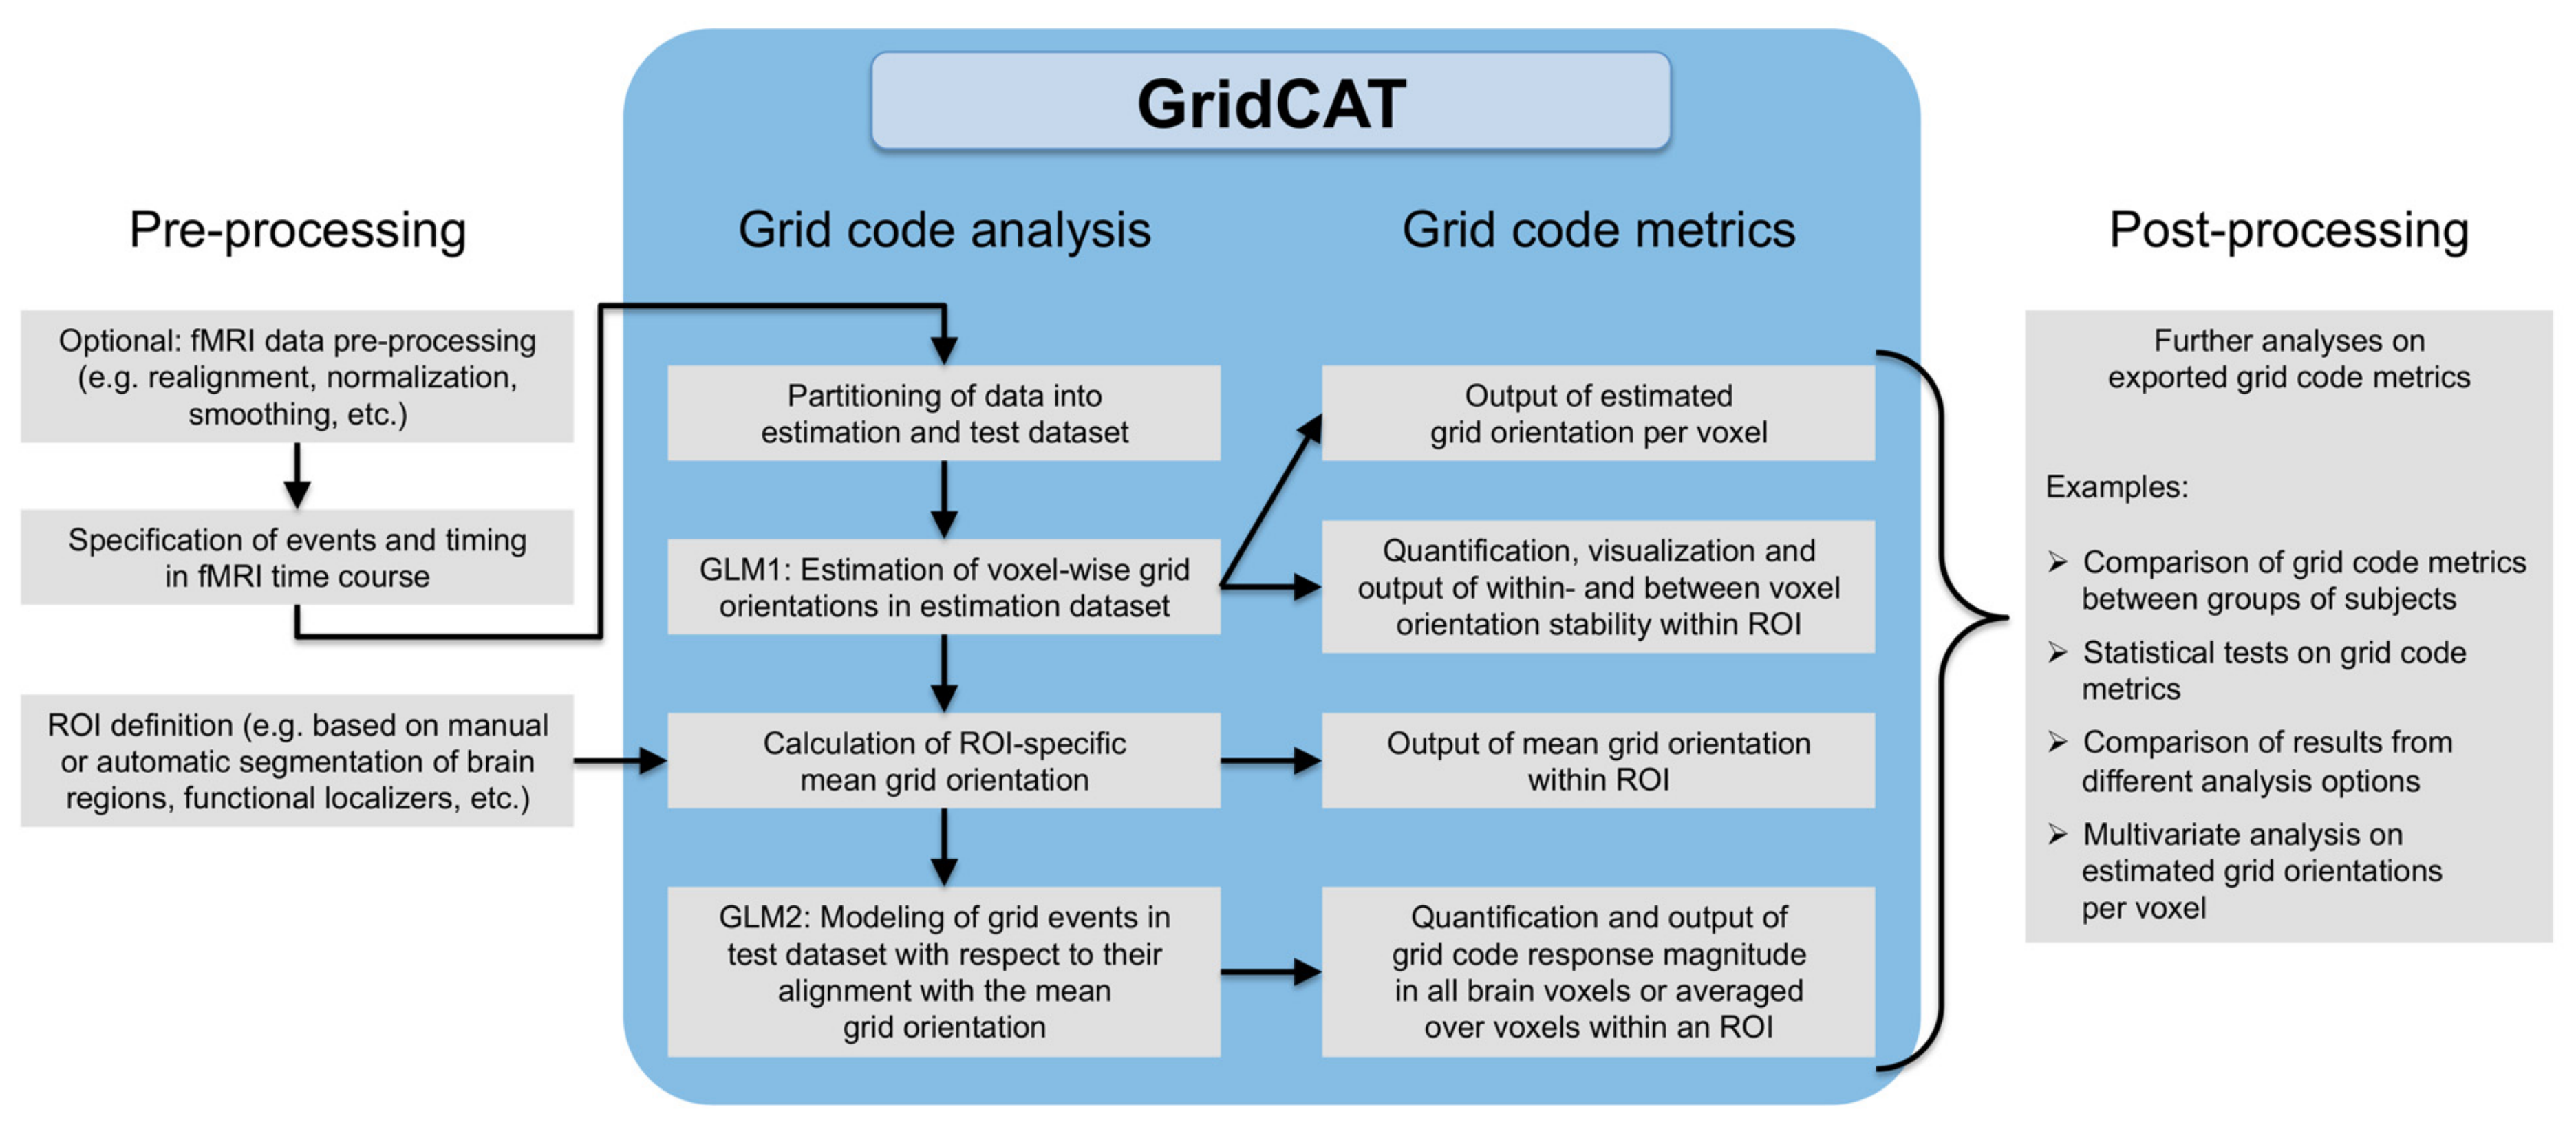
\includegraphics[width=0.8\linewidth]{gridcat_tabular.png}
    \caption{General pipeline for GridCAT. Figure adapted from \cite{stangl_gridcat_2017}}
    \label{fig:gridcat_intro}
\end{figure}

As described in the data subsection, 6 runs of open field and 6 runs of barrier environment fMRI was used. Each set of runs was loaded separately into GridCAT, along with the corresponding event tables indicating the time points corresponding to binary events ‘Question’ and ‘Translation’. For GLM training and validation, half of the runs were assigned to each category based on the odd-even nature of the run number. Thus, GLM1 is calculated first using two parametric regressors:  $ \beta_1 = \sin(6 \cdot \alpha_t)$ and  $\beta_2 = \cos(6 \cdot \alpha_t)$, where $\alpha_t$ is an individual grid event angle. This provides information on the voxel-wise grid orientation in the dataset. In particular, the symmetry information for the data should be provided here. In the case of OF, it is a six-fold symmetry whereas it is a four-fold symmetry in the case of BA \cite{he_environmental_2019}. 

As mentioned in the preprocessing steps, the right entorhinal cortex (REC) was consistently used as the ROI mask. Using the mask, GLM2 is now calculated, modeling grid events in the test data set by considering their alignment with the mean grid orientation within the ROI. The mean grid orientation is calculated using the previously mentioned parametric regressors: 

\begin{equation}
\text{$\varphi$} = \frac{\arctan(\bar{\beta_1}/\bar{\beta_2})}{6}
\end{equation}

\noindent This calculation provides information about the magnitude of alignment for the 6-fold symmetry. Going further, a parametric modulation regressor is used to measure the sinusoidal activity of the grid cells with respect to the symmetry. The cosine of the difference between the angle of the grid event ($\alpha_t$) and the mean grid orientation ($\varphi$) is used for this purpose, where it is 1 for perfect alignment once every $60^{\circ}$ for 6-fold symmetry: 
\begin{equation}
\text{Parametric Regressor} = \cos\left( 6 \cdot (\alpha_t - \varphi) \right) \\
\end{equation}


\noindent GridCAT can be used to produce multiple metrics and visualizations as part of the GUI. For the current study, the coherence of the between-voxel orientation within the ROI, and the coherence of the within-voxel orientation within the ROI (voxel stability) were plotted and interpreted. The principal reason for using GridCAT is its intuitive GUI and well-documented manual. However, it is inherently based on using simple GLM techniques, which require BOLD signal processing. 

\subsubsection{\textbf{CNN}}
\noindent \textbf{3D-CNN Architecture}
\noindent A 3D convolutional neural network (3D-CNN) was designed to predict grid cell alignment within a 0–360° range. The model architecture consisted of two 3D convolutional layers, each with a kernel size of 3, followed by max-pooling layers with a kernel size of 2 and a stride of 2. The first convolutional layer utilized 64 filters, while the second applied 128 filters. The extracted features were passed through two fully connected layers, with the first dynamically sized to accommodate the flattened output of the convolutional layers, and the second outputting two values to represent the sine and cosine of the grid cell alignment angle. ReLU activation functions were applied after each convolutional and fully connected layer, and dropout regularization (rate = 0.3) was incorporated in the first fully connected layer to reduce the risk of overfitting. The final output layer employed linear activation to predict continuous values for alignment representation.\\

\noindent \textbf{1D-CNN Architecture}\\
To capture the spatial dependencies within the fMRI voxel activation patterns and predict the continuous alignment scores, we developed a 1D-CNN model. The architecture is designed to efficiently extract local spatial features from the high-dimensional input data and map them to the target variable. A schematic overview of the network architecture is presented in Figure \ref{fig:1dCNNarch}. The network processes the normalized voxel activation vector \(\mathbf{X} \in \mathbb{R}^{N}\) as input, where each element represents the BOLD signal intensity of a voxel at a given time point. The architecture begins with a convolutional layer employing 32 filters with a kernel size of 3, utilizing the Rectified Linear Unit (ReLU) activation function to capture local spatial patterns in the data. This is followed by a max-pooling layer with a pool size of 2 to reduce dimensionality and focus on the most salient features, and a dropout layer with a rate of 0.3 to prevent overfitting. A second convolutional layer with 64 filters and the same kernel size further extracts higher-level features, followed by another max-pooling and dropout layer. The extracted features were flattened into a one-dimensional vector and passed through a fully connected layer with 128 neurons and ReLU activation to integrate the learned representations. A final dropout layer with a rate of 0.5 is applied before the output layer, which consists of a single neuron with a linear activation function to predict the continuous alignment score, \(\mathbf{y}\). This architecture is designed to capture complex spatial patterns in the fMRI data while incorporating regularization techniques to enhance generalization, thereby facilitating accurate regression modeling of neural responses.\\

\begin{figure}
    \centering
    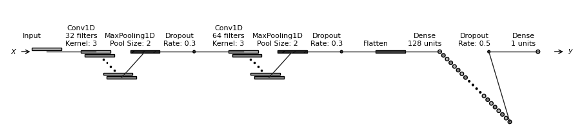
\includegraphics[width=1\linewidth]{CNNArch2.png}
    \caption{Schematic representation of the 1D-CNN architecture used for predicting alignment scores from fMRI voxel activation vectors.}
    \label{fig:1dCNNarch}
\end{figure}

\noindent \textbf{Training Procedure and Validation Techniques}\\
The 1D-CNN model was trained to predict continuous alignment scores by minimizing the Mean Squared Error (MSE) loss function:
\begin{equation}
\mathcal{L} = \frac{1}{T} \sum_{t=1}^{T} \left( y_t - \hat{y}_t \right)^2,
\end{equation}


\noindent where \( y_t \) is the true alignment score, \( \hat{y}_t \) is the predicted score, and \( T \) is the number of training samples. We utilized the Adam optimizer with a learning rate of \( 1 \times 10^{-4} \) to efficiently handle sparse gradients and adaptively adjust learning rates during training. The model was trained over 200 epochs with a batch size of 32, balancing computational efficiency with the ability to capture complex patterns in the data. The dataset was divided into training and validation sets using an 80:20 split, employing hold-out validation to evaluate the model's generalization performance on unseen data. Throughout the training process, we monitored both the training and validation MSE and Mean Absolute Error (MAE) to assess learning progression and detect any signs of overfitting or underfitting. Learning curves were plotted to visualize the trajectory of these metrics over the epochs, providing insights into the model's convergence behavior.

To further assess the model's predictive performance and its ability to capture the cyclical nature of the stimulus data, we analyzed the distribution of prediction errors and visualized the predicted alignment scores relative to stimulus orientations. We generated a histogram of normalized absolute prediction errors, illustrating the frequency of errors from zero (indicating perfect predictions) to one (indicating maximum possible errors), providing an overview of the model's accuracy. Additionally, we plotted the predicted alignment scores on a circular graph corresponding to the orientation angles of the stimuli. In this visualization, the angle of each point represents the stimulus orientation, the radius corresponds to the predicted alignment score, and the color indicates the magnitude of the prediction error. This circular plot enabled us to evaluate how effectively the model captured the inherent periodicity of the data, which is crucial for accurately modeling neural responses to different stimulus orientations. By employing these comprehensive evaluation strategies, we ensured a thorough assessment of the model's performance, focusing on both prediction accuracy and generalization capability. This approach allowed us to confirm the model's effectiveness in capturing the complex relationships between voxel activation patterns and alignment scores.

\subsubsection{\textbf{1D-CNN-LSTM}}
\noindent \textbf{1D-CNN-LSTM Architecture}\\
The 1D-CNN-LSTM architecture combines convolutional and recurrent neural networks to capture both spatial and temporal patterns in the BOLD signal data (see Figure \ref{fig:1D-CNN-LSTM}). The model processes sequences of voxel activation vectors with shape \((\text{timesteps}, N)\), where \(N\) is the total number of voxels. It begins with three 1D convolutional layers with 16, 32, and 64 filters respectively, each with a kernel size of 3, ReLU activation, and 'same' padding to preserve the temporal dimensions. These layers extract local spatial features from the voxel data at each time step. Following the convolutional layers, the model includes three stacked LSTM layers with 64, 32, and 16 units respectively, all using ReLU activation and configured to return sequences. This setup enables the model to learn complex temporal dependencies across the sequences. Finally, two TimeDistributed dense layers are applied: the first with 100 neurons and ReLU activation, and the second with a single neuron to predict the continuous alignment score at each time step. This model is designed to capture the spatiotemporal dynamics of neural responses associated with different stimulus orientations by leveraging convolutional layers for spatial feature extraction and LSTM layers for temporal modeling.\\

\begin{figure}
    \centering
    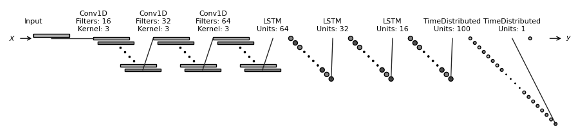
\includegraphics[width=1\linewidth]{hybrid2.png}
    \caption{Schematic representation of the 1D-CNN-LSTM architecture used for predicting alignment scores from
fMRI voxel activation vectors.}
    \label{fig:1D-CNN-LSTM}
\end{figure}

\noindent \textbf{Training Procedure and Validation Techniques}\\
The training and validation processes for the 1D-CNN-LSTM model were identical to those employed for the 1D-CNN model described earlier. Specifically, the model was trained to predict continuous alignment scores by minimizing the MSE loss function using the Adam optimizer with a learning rate of \(1 \times 10^{-4}\). Training was conducted over 200 epochs with a batch size of 32, utilizing an 80:20 train-validation split to evaluate the model's generalization performance on unseen data. Performance was assessed using both MSE and MAE, and learning curves were monitored to track the progression of these metrics and detect any signs of overfitting or underfitting. Additionally, the distribution of prediction errors and the alignment of predicted scores with stimulus orientations were analyzed to ensure the model effectively captured the cyclical nature of the data. These comprehensive evaluation strategies ensured a thorough assessment of the model's predictive accuracy and its ability to generalize the learned spatiotemporal patterns in neural responses.


% Section: Results
\section{Results}

\subsection{\textbf{GridCat Performance}}
\label{sec:results}

Based on previous work by \cite{he_environmental_2019}, GridCAT was used to analyze the data derived from subject s05. The runs were separated into OF and BA, and the between-voxel orientation coherence within ROI was visualized for analysis. The figures appear like polar plots with histograms depicting the frequency of the alignment angle, and thus, a stronger alignment is when the histograms are more clustered. Similarly, the mean orientation can also be visualized, with and without considering for the amplitude-based weighting of voxels. This is indicated by the two different colored arrows. The statistical test for non-uniformity in polar cases is the Rayleigh test. In all the cases, the p-value was 0, indicating a non-uniformity. This indicates a preference towards a particular orientation. This visualization was performed for both the 6-fold OF and 4-fold BA runs.

In the Figure \ref{fig:combined_alignment}, in the case of OF, there is strong alignment when the subject is undergoing translation. However, in the case of questioning when the subject is also performing a cognitive task, we note a marked reduction of grid cell alignment. Overall, among all the runs involving translation, there is a consistent clustering of grid cells.

\begin{figure}[h]
    \centering
    % First row of subfigures
    \begin{subfigure}[b]{0.3\textwidth}
        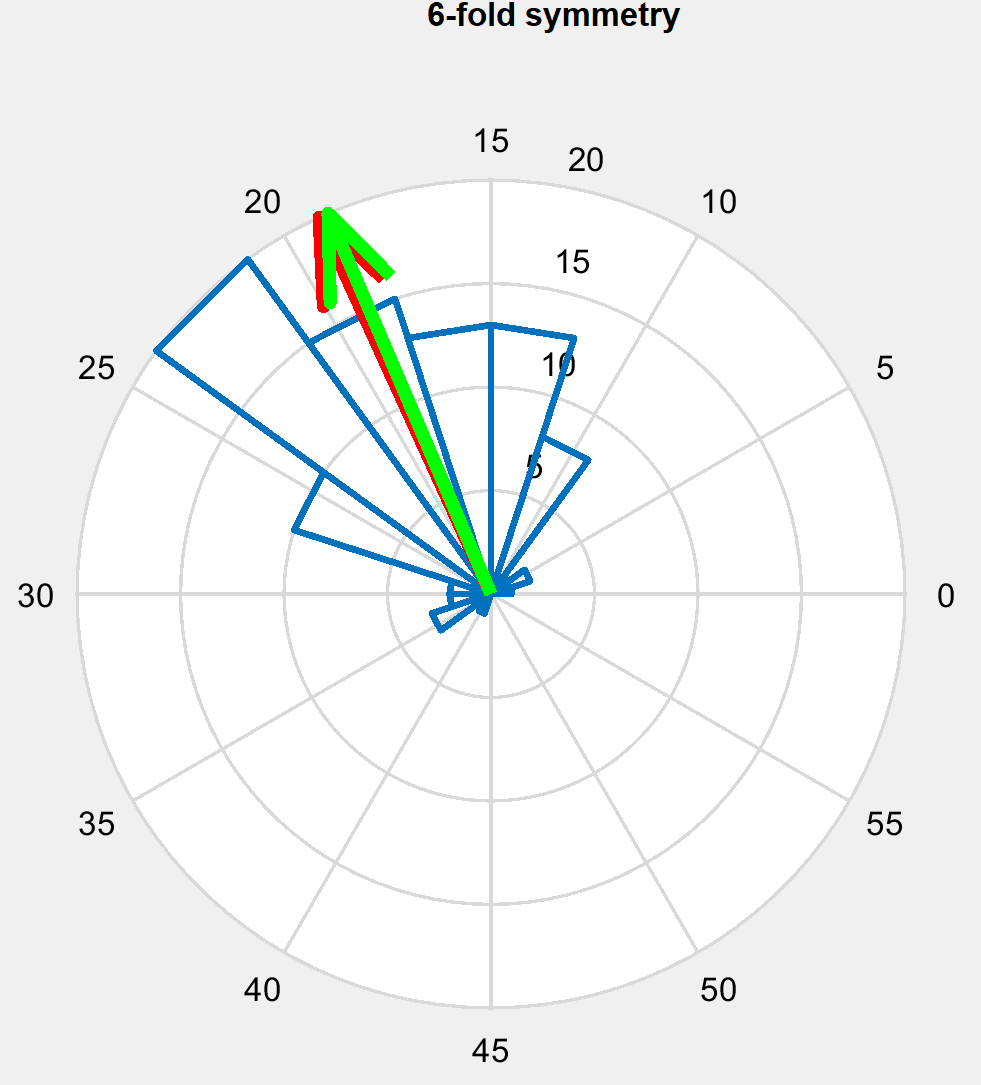
\includegraphics[width=\linewidth]{alignment_trans_OF.png}
        \caption{Translation - OF}
        \label{fig:alignment_trans_OF}
    \end{subfigure}
    \hfill
    \begin{subfigure}[b]{0.3\textwidth}
        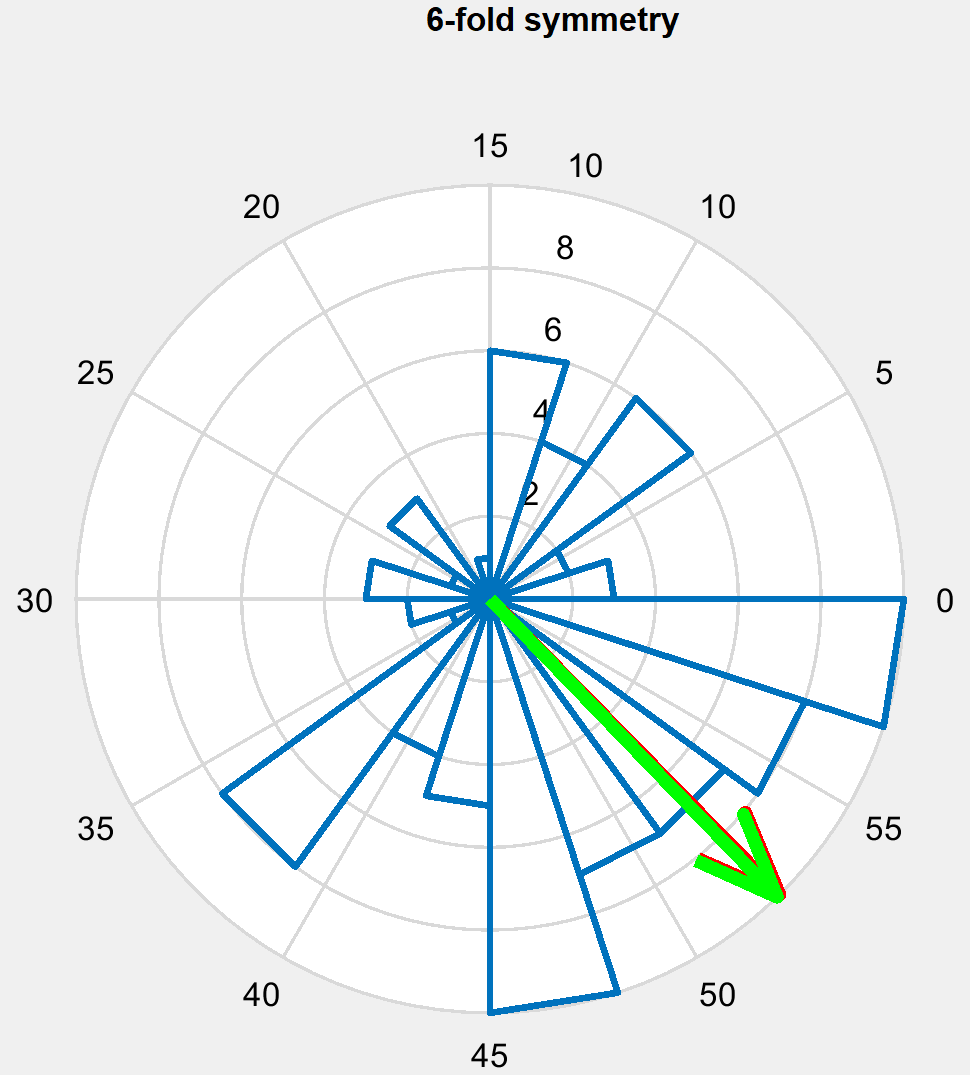
\includegraphics[width=\linewidth]{alignment_question_OF.png}
        \caption{Question - OF}
        \label{fig:alignment_ques_OF}
    \end{subfigure}
    \hfill
    \begin{subfigure}[b]{0.3\textwidth}
        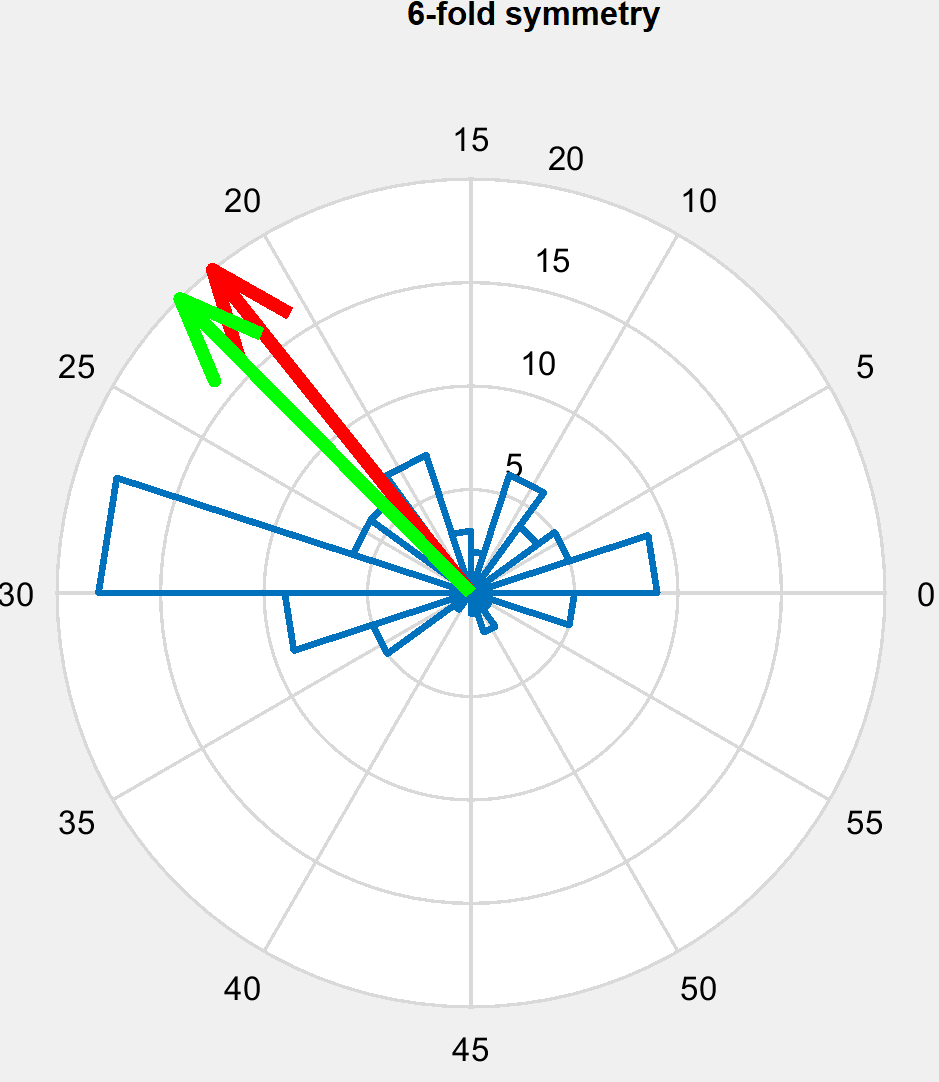
\includegraphics[width=\linewidth]{alignment_trans_ALL_OF.png}
        \caption{Translation - All runs - OF}
        \label{fig:alignment_trans_ALL_OF}
    \end{subfigure}
    
    \vspace{0.5cm}
    % Second row of subfigures
    \begin{subfigure}[b]{0.3\textwidth}
        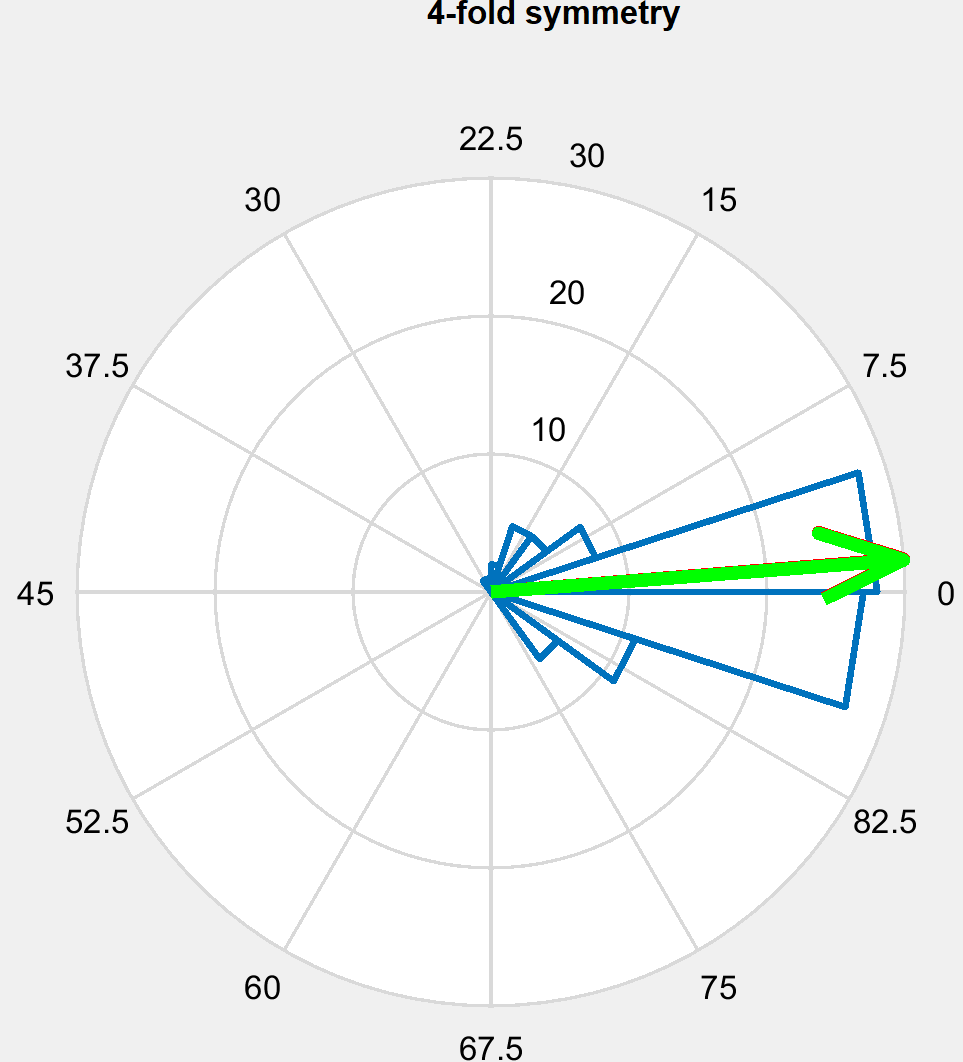
\includegraphics[width=\linewidth]{alignment_trans_BA.png}
        \caption{Translation - BA}
        \label{fig:alignment_trans_BA}
    \end{subfigure}
    \hfill
    \begin{subfigure}[b]{0.3\textwidth}
        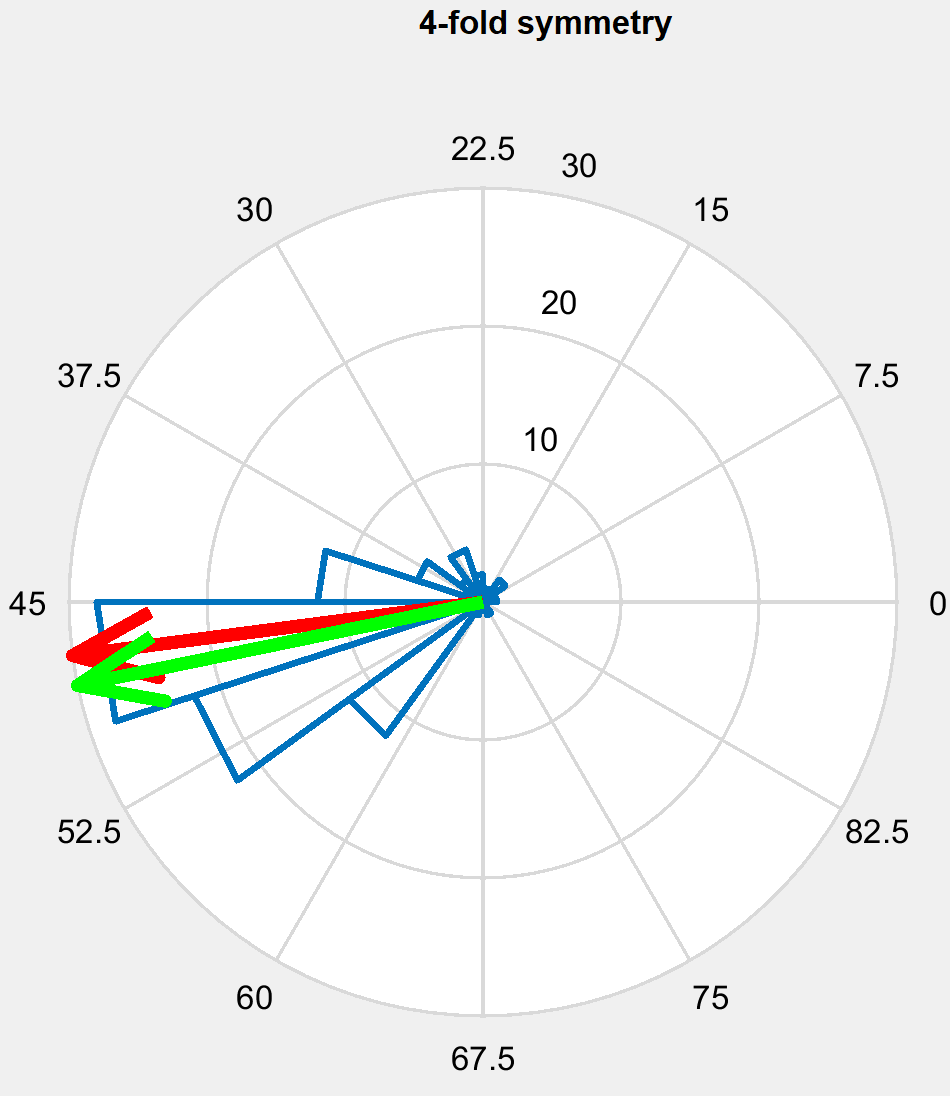
\includegraphics[width=\linewidth]{alignment_question_BA.png}
        \caption{Question - BA}
        \label{fig:alignment_ques_BA}
    \end{subfigure}
    \hfill
    \begin{subfigure}[b]{0.3\textwidth}
        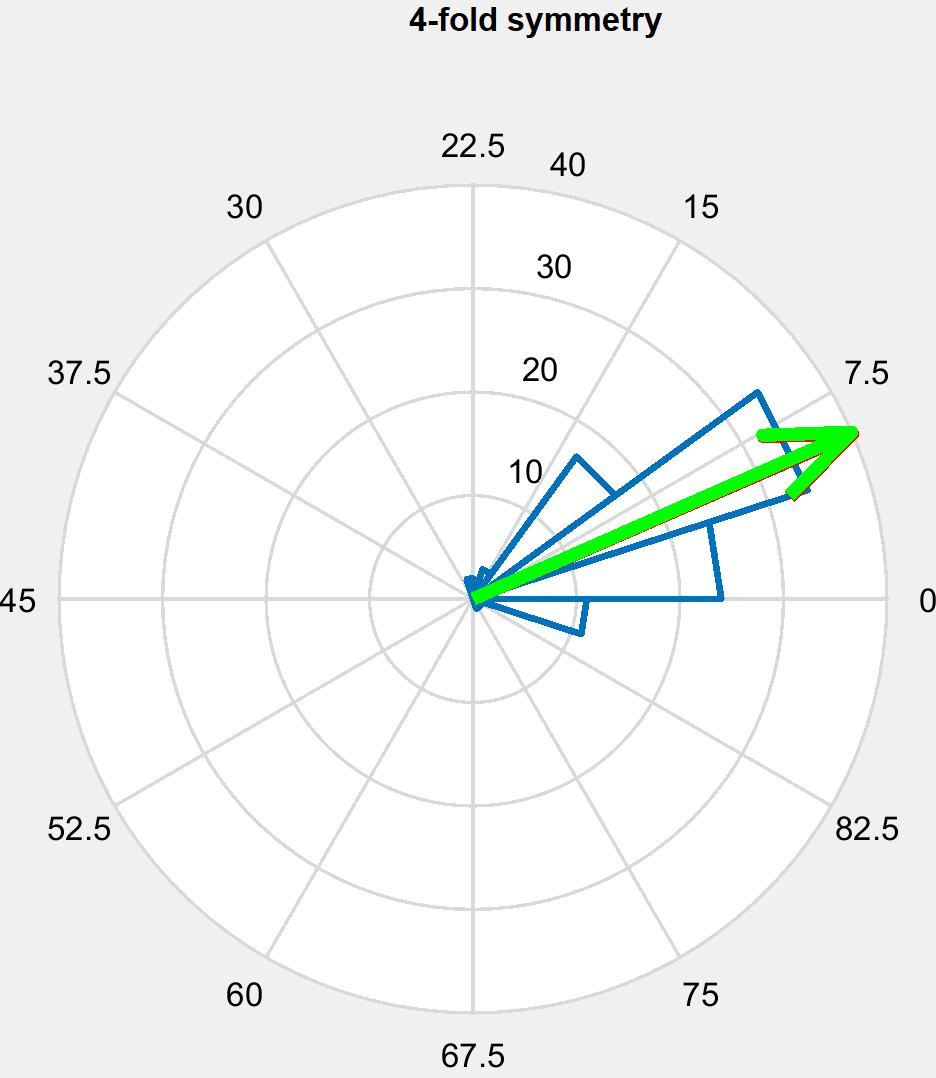
\includegraphics[width=\linewidth]{alignment_trans_ALL_BA.png}
        \caption{Translation - All runs - BA}
        \label{fig:alignment_trans_ALL_BA}
    \end{subfigure}

    \caption{Combined sub-figures for alignment study. The green arrow indicates the mean grid orientation with amplitude-based weighting of voxels, while the red arrow indicates the mean grid orientation without amplitude-based weighting of voxels. Note that the difference between the two is generally not significant, indicating that the voxels all generally have similar amplitude within the ROI.}
    \label{fig:combined_alignment}
\end{figure} 

In the case of grid cell alignment for BA, we note a strong alignment in the case of translation as well as questioning, which is different from the observations in the case of OF runs. There is also a stronger alignment overall, in all the translation runs. We also note that the mean direction of alignment in the translation and questioning are markedly flipped in both the cases of OF and BA, despite there being a lower alignment in OF questioning case. This is discussed further in Section \ref{sec:discussion}.

The within-voxel orientation coherence within ROI was also visualized in Figure \ref{fig:stability_voxels}. The plots indicate concentric circles with green connections indicating voxels which had stable orientation within the threshold. This indicates the consistency of the runs. The proportion of stable voxels indicate a sustained and consistent orientation from the grid cells during the tasks. The threshold varies between OF and BA, as it is by default considered to be the right angle divided by the number of folds of symmetry.

In the case of OF, there is a strong stability in the runs while translation is being performed. As visualized, the best stability can be seen between run 1 and run 3 considering a threshold of $15^\circ$ at 78.02\%. However, the stability of translation and question across the same run 1 at the same threshold is significantly lower at 34.07\%. This can be explained by the flipping of the mean orientation as noted in the between-voxel alignment plots.

In the case of BA, the threshold is increased to $22.5^\circ$ due to the reduction in the folds of symmetry. The best stability in translation was noted between run 4 and run 6 at 76.6\%. Comparing translation and question, between run 4 and run 6, the stability falls down to 11.7\%. This drop in stability between translation and questioning is consistent in both OF and BA, indicating a change in orientation within the voxels while performing the pure translation task and the cognitive questioning task.\\

\begin{figure}
    \centering
    % First row of subfigures
    \begin{subfigure}[b]{0.45\textwidth}
        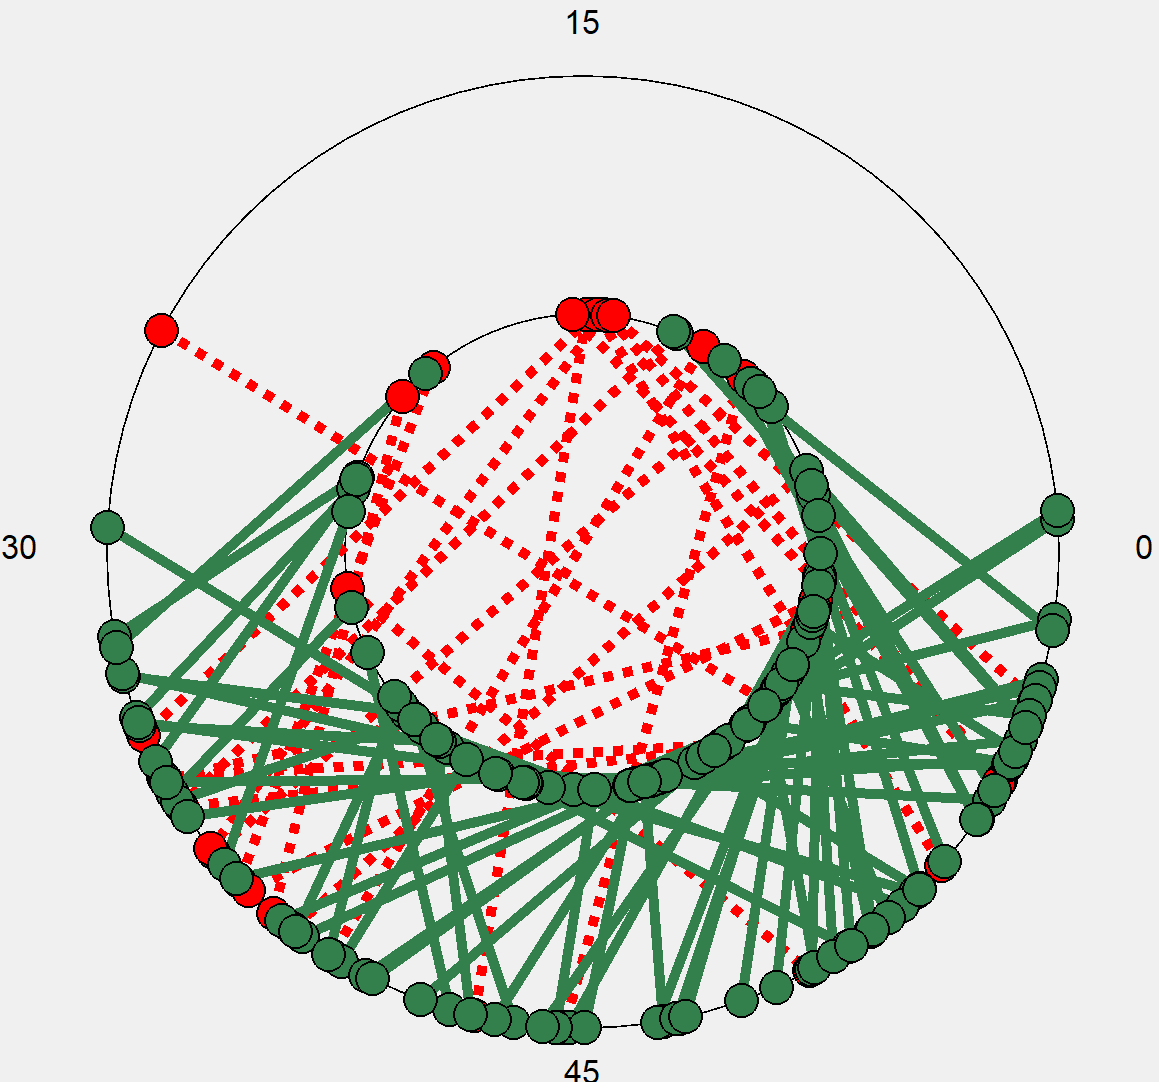
\includegraphics[width=\linewidth]{stable_OF_run_only.png}
        \caption{Translation: R1 and R3: 78.02\%@15°}
        \label{fig:stable_OF_run_only}
    \end{subfigure}
    \hspace{0.03\textwidth} % Reduced spacing
    \begin{subfigure}[b]{0.45\textwidth}
        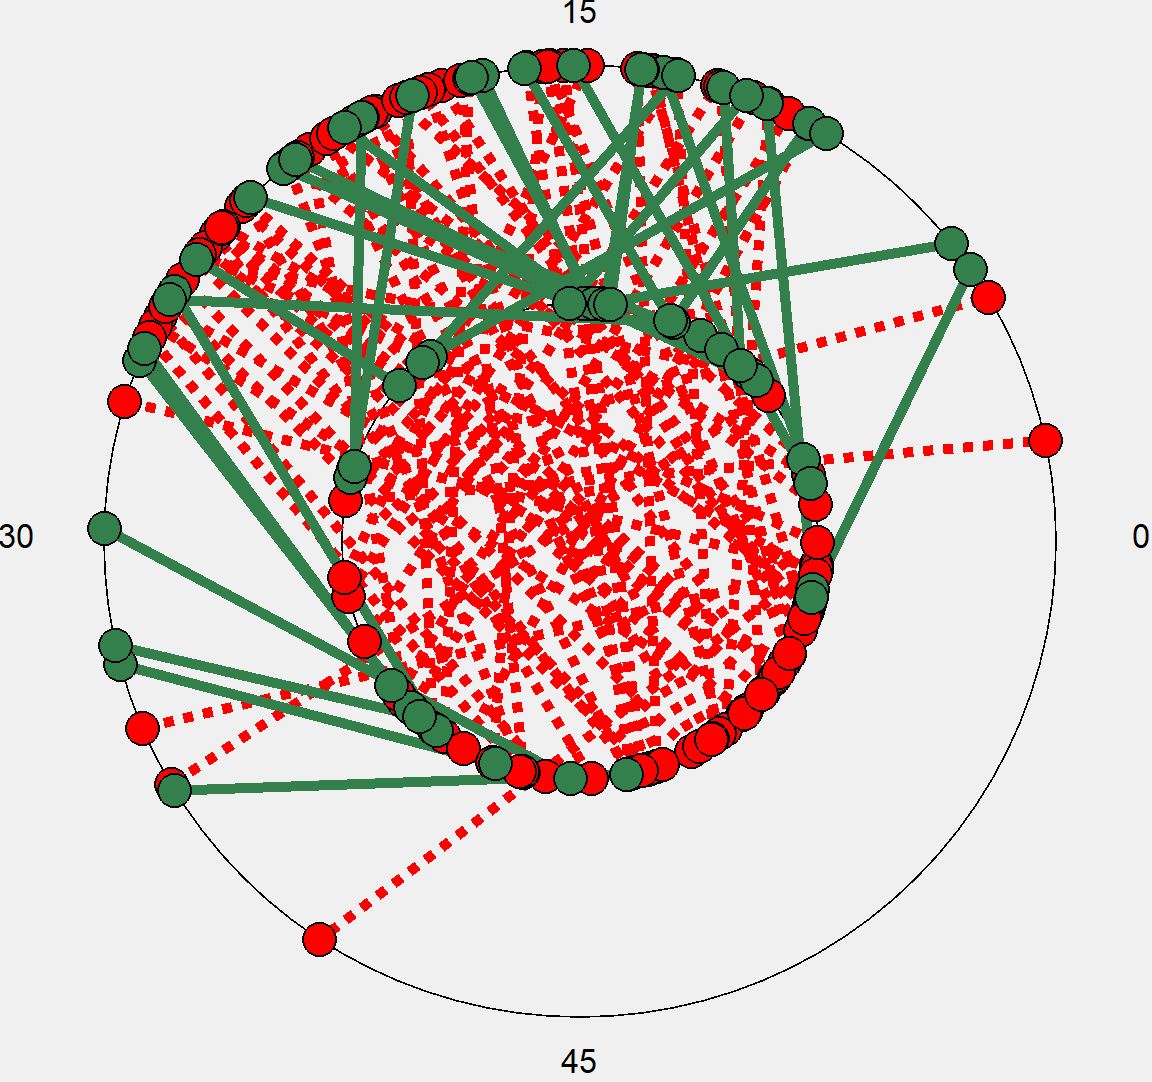
\includegraphics[width=\linewidth]{stable_OF_run_ques.png}
        \caption{Translation:R1 and Question:R1 34.07\%@15°}
        \label{fig:stable_OF_run_ques}
    \end{subfigure}
    
    \vspace{0.2cm} % Reduced vertical spacing
    % Second row of subfigures
    \begin{subfigure}[b]{0.45\textwidth}
        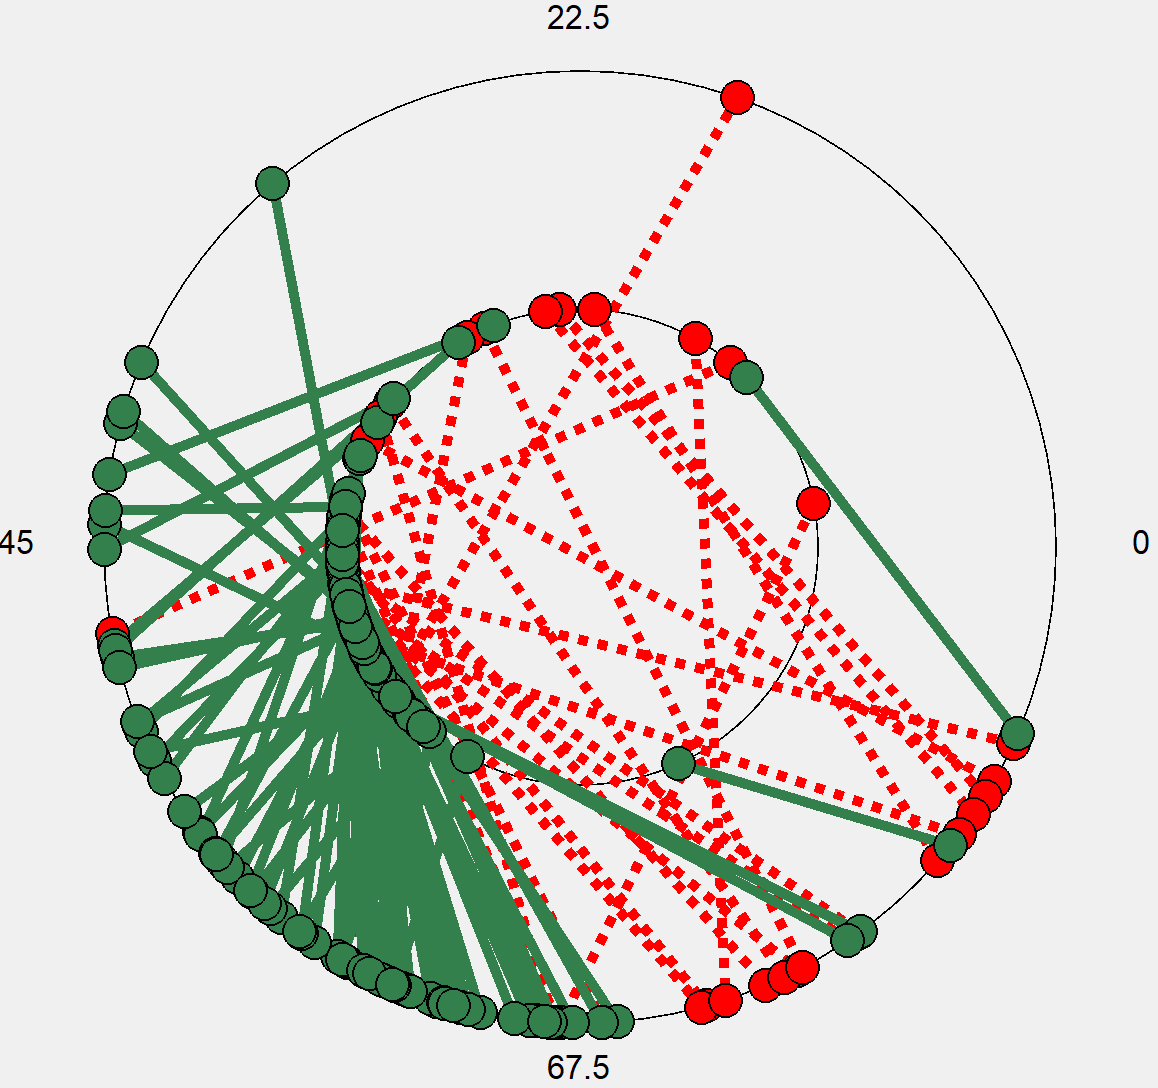
\includegraphics[width=\linewidth]{stable_BA_run_only.png}
        \caption{Translation: R4 and R6: 76.6\%@22.5°}
        \label{fig:stable_BA_run_only}
    \end{subfigure}
    \hspace{0.03\textwidth} % Reduced spacing
    \begin{subfigure}[b]{0.45\textwidth}
        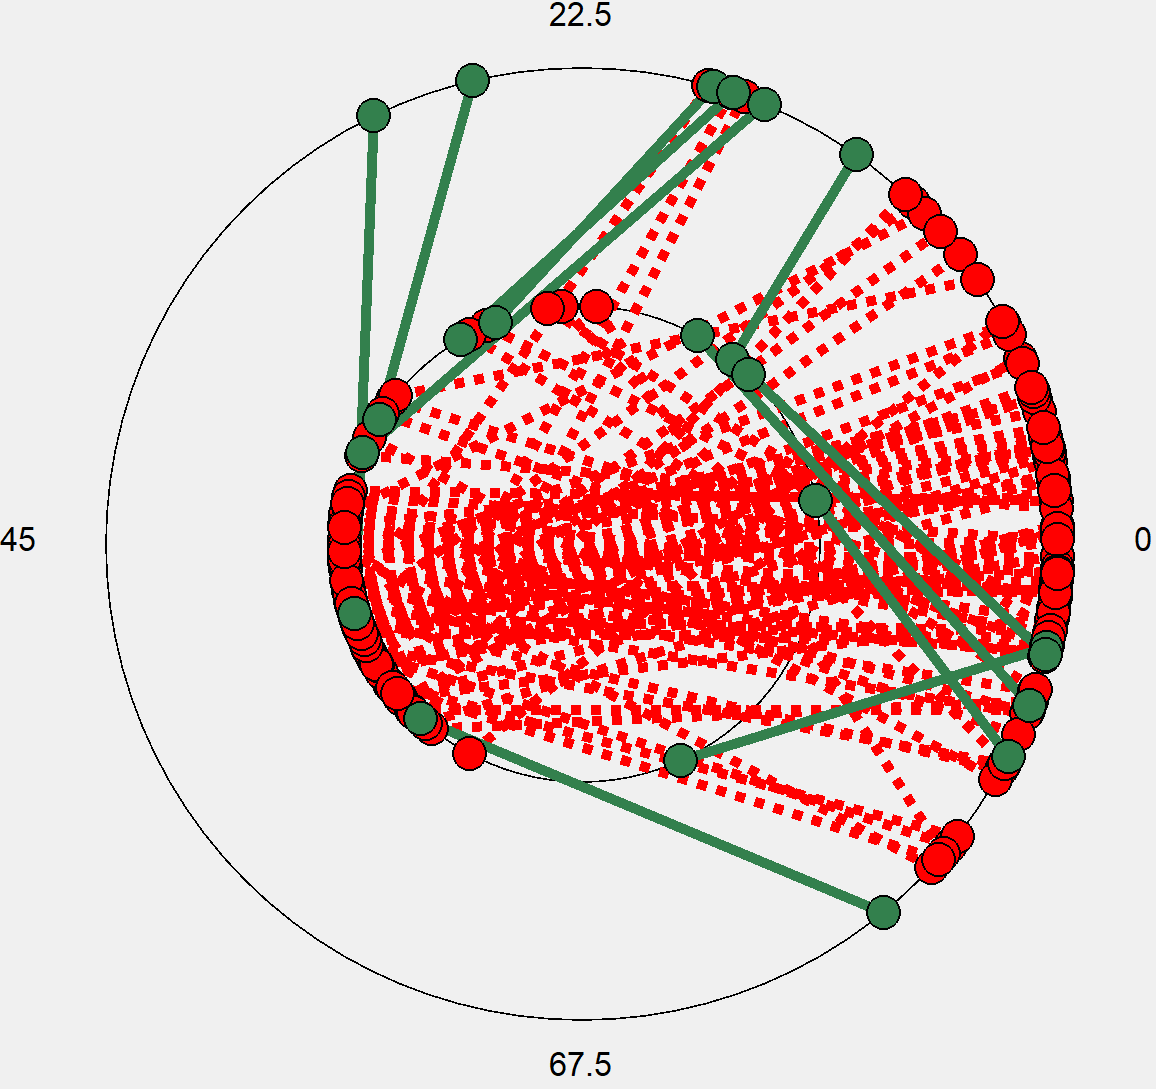
\includegraphics[width=\linewidth]{stable_BA_run_quest.png}
        \caption{Translation:R4 and Question:R6: 11.7\%@22.5°}
        \label{fig:stable_BA_run_ques}
    \end{subfigure}
    \caption{Within-voxel alignment cohesion plots, where the concentric circles represent the orientation of individual voxels in each run. The specific voxels are indicated by the points on the circles and joined by lines, where the green line indicates stability within the threshold. Note the difference in the thresholds between OF and BA.}
    \label{fig:stability_voxels}
\end{figure}

\subsection{\textbf{3D CNN Performance}}
The 3D CNN model demonstrated low predictive accuracy, achieving approximately 5.5\% on the training set and 4.2\% on the validation set when estimating angles (0–360 degrees) from right entorhinal cortex (EC) images. Various optimization and hyperparameter tuning strategies, including adjustments to the learning rate (1e-3, 1e-4, 1e-5), batch sizes (2, 4, and 8), and regularization through weight decay (1e-5), were explored. Data augmentation techniques, such as random horizontal and vertical flips, and attempts to increase the model complexity (doubling the number of filters and parameters) were also tested. However, these modifications failed to significantly improve performance. Consequently, we decided to convert the voxels into a 1D BOLD signal and measure alignments of the grid cells.



\subsection{\textbf{1D-CNN Performance}}
The 1D-CNN model was trained for over 200 epochs to predict orientation alignment scores from voxel activation patterns. The training and validation metrics at every 50 epochs are summarized in Table~\ref{tab:1dcnnmodel_performance}.
\begin{figure}
    \centering
    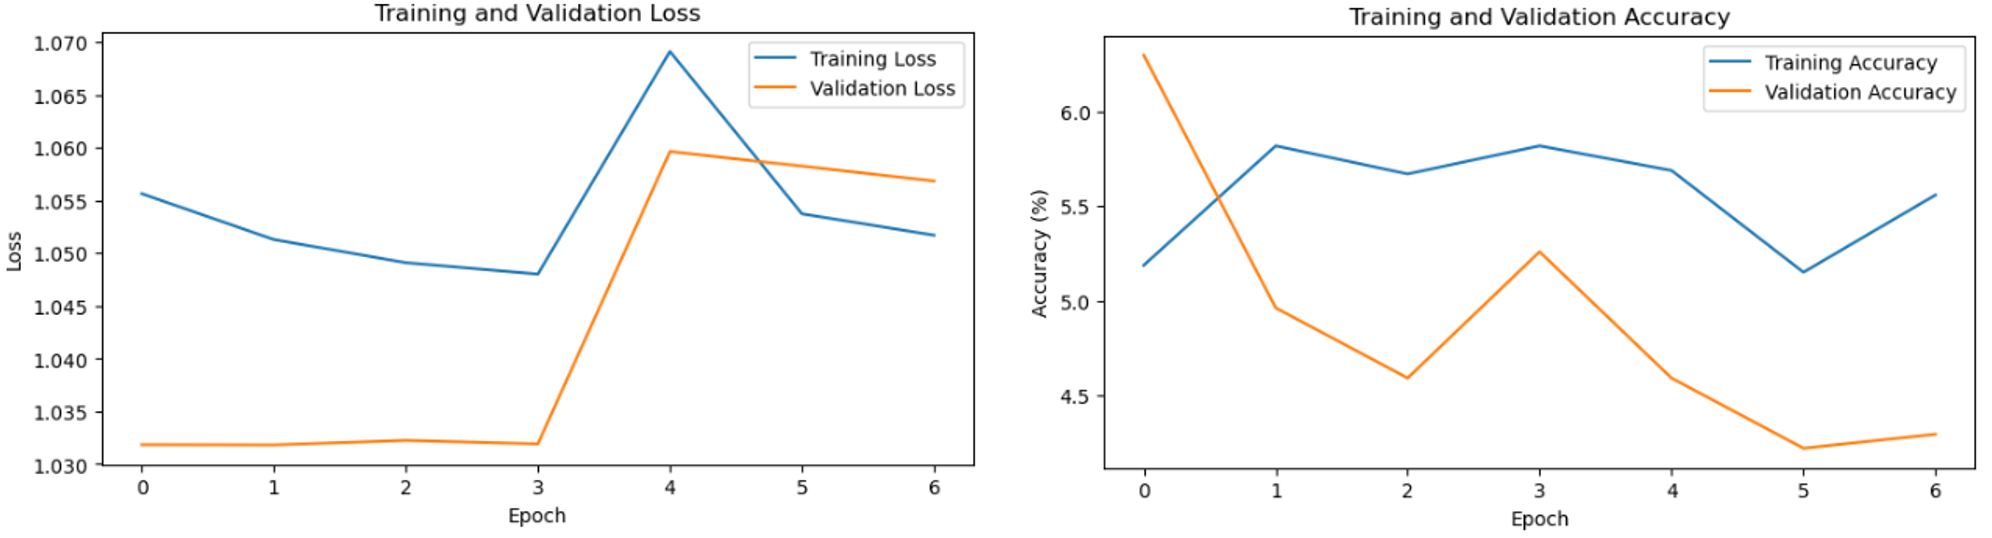
\includegraphics[width=1\linewidth]{final_report/3D_CNN_results.png}
    \caption{Learning Curves of the 3D-CNN Model 6 Epochs with early stopping. The left subplot displays the training and validation loss, while the right subplot illustrates the training and validation accuracies.}
    \label{fig:3DCNN}
\end{figure}
\subsubsection{Training and Validation Assessment}
As illustrated in Figure \ref{fig:updated1Dmse}, the 1D-CNN model exhibited a steady decrease in training loss over 200 epochs, with the training Mean Squared Error (MSE) reducing from 0.5515 to 0.3981 and the training Mean Absolute Error (MAE) decreasing from 0.6643 to 0.5429. This consistent decline indicates the model's effectiveness in learning and capturing patterns within the training neural data associated with specific orientation alignments. However, the validation metrics presented a contrasting trend. The validation MSE decreased from 0.8102 at epoch 1 to approximately 0.5622 by epoch 30 but plateaued thereafter, showing no significant improvement despite continued training. Similarly, the validation MAE remained relatively stable, marginally decreasing from 0.6619 to 0.6504 over the entire training period. This plateau suggests that the model's ability to generalize learned patterns to unseen data is limited, likely due to overfitting.

\begin{table}[H]
\centering
\begin{tabular}{|c|c|c|c|c|}
\hline
\textbf{Epoch} & \textbf{Training MSE Loss} & \textbf{Training MAE} & \textbf{Validation MSE Loss} & \textbf{Validation MAE} \\ \hline
1              & 0.5515                     & 0.6643                & 0.5472                       & 0.6619                  \\ \hline
50             & 0.5270                     & 0.6475                & 0.5432                       & 0.6576                  \\ \hline
100            & 0.5084                     & 0.6334                & 0.5423                       & 0.6526                  \\ \hline
150            & 0.4586                     & 0.5916                & 0.5412                       & 0.6481                  \\ \hline
200            & 0.3981                     & 0.5429                & 0.5499                       & 0.6504                  \\ \hline
\end{tabular}
\caption{Mean Squared Error (MSE) loss and Mean Absolute Error (MAE) Performance Metrics for Training and Validation of a 1D-CNN Model Over 200 Epochs.}
\label{tab:1dcnnmodel_performance}
\end{table}


\begin{figure}
    \centering
    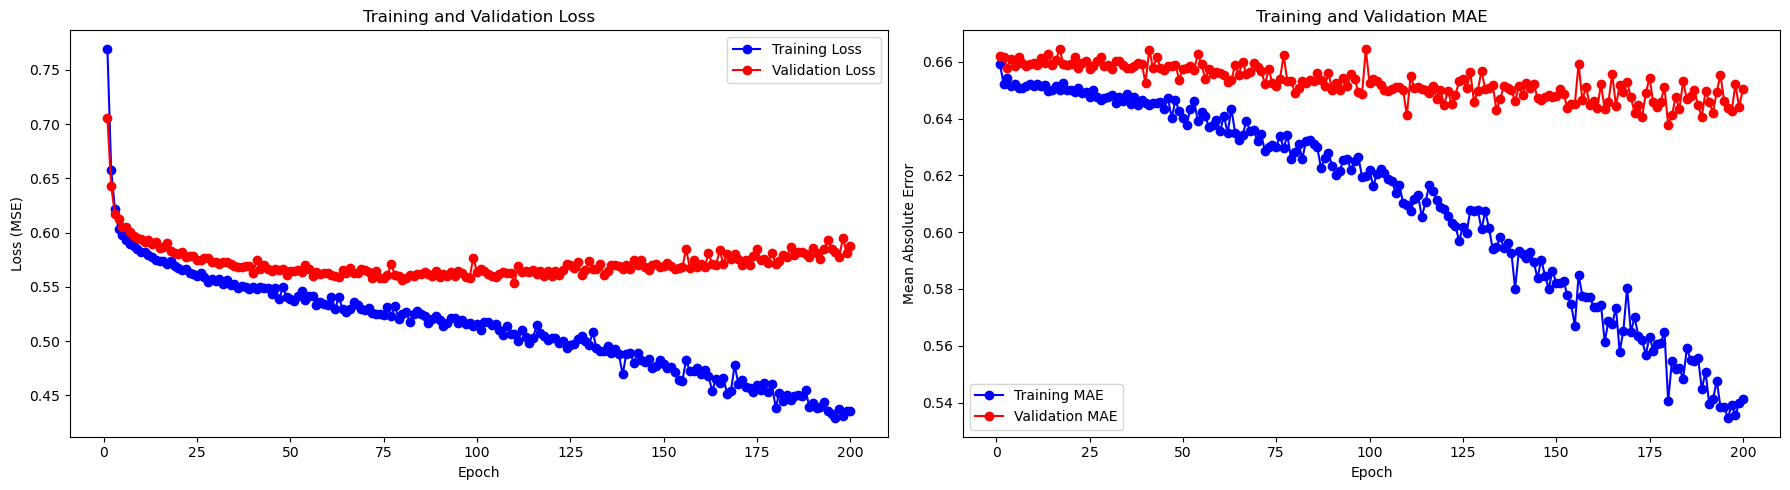
\includegraphics[width=1\linewidth]{MSE_MAE_1D.png}
    \caption{Learning Curves of a 1D-CNN Model Over 200 Epochs. The left subplot displays the training and validation MSE loss, while the right subplot illustrates the training and validation MAE.}
    \label{fig:updated1Dmse}
\end{figure}



\subsection{\textbf{1D-CNN-LSTM Performance}}

 To further enhance prediction accuracy, we developed the 1D-CNN-LSTM model by integrating Long Short-Term Memory layers into the existing 1D-CNN architecture. This hybrid approach leverages spatial features from voxel activation patterns and captures temporal dependencies across 10 time steps to predict orientation alignment scores. The model was trained for over 200 epochs, with training and validation metrics recorded every 50 epochs and summarized in Table~\ref{tab:1D-CNN-LSTM-model_performance}.

\subsubsection{Training and Validation Assessment}

As illustrated in Figure \ref{fig:mseless_mae1DCNN-LSTM}, the 1D-CNN-LSTM model exhibited a gradual decrease in training loss over 200 epochs, with the training MSE reducing from 0.5471 at epoch 1 to 0.4692 at epoch 200. Similarly, the training MAE decreased from 0.6523 to 0.5961 over the same period. This consistent decline indicates the model's effectiveness in learning and capturing patterns within the training neural data associated with specific orientation alignments.\\


\begin{table}[h]
\centering
\begin{tabular}{|c|c|c|c|c|} \hline
\textbf{Epoch} & \textbf{Training MSE Loss} & \textbf{Training MAE} & \textbf{Validation MSE Loss} & \textbf{Validation MAE} \\ \hline
1              & 0.5471                     & 0.6523                & 0.5692                       & 0.6730                  \\ \hline
50             & 0.5198                     & 0.6352                & 0.5583                       & 0.6633                  \\ \hline
100            & 0.5055                     & 0.6256                & 0.5572                       & 0.6568                  \\ \hline
150            & 0.4976                     & 0.6207                & 0.5515                       & 0.6554                  \\ \hline
200            & 0.4692                     & 0.5961                & 0.5466                       & 0.6484                  \\ \hline
\end{tabular}
\caption{ Mean Squared Error (MSE) loss and Mean Absolute Error (MAE) Performance Metrics for Training and Validation of a 1D-CNN-LSTM Model Over 200 Epochs.}
\label{tab:1D-CNN-LSTM-model_performance}
\end{table}


However, the validation metrics presented a modest improvement. The validation MSE decreased from 0.5692 at epoch 1 to 0.5466 by epoch 200, while the validation MAE decreased from 0.6730 to 0.6484. Although there is a slight downward trend in validation MSE loss and MAE, the improvements are less pronounced compared to the training metrics. This suggests that while the model is learning effectively on the training data, its ability to generalize to unseen data is somewhat limited. The relatively stable validation metrics may indicate mild overfitting.\\

\begin{figure}
    \centering
    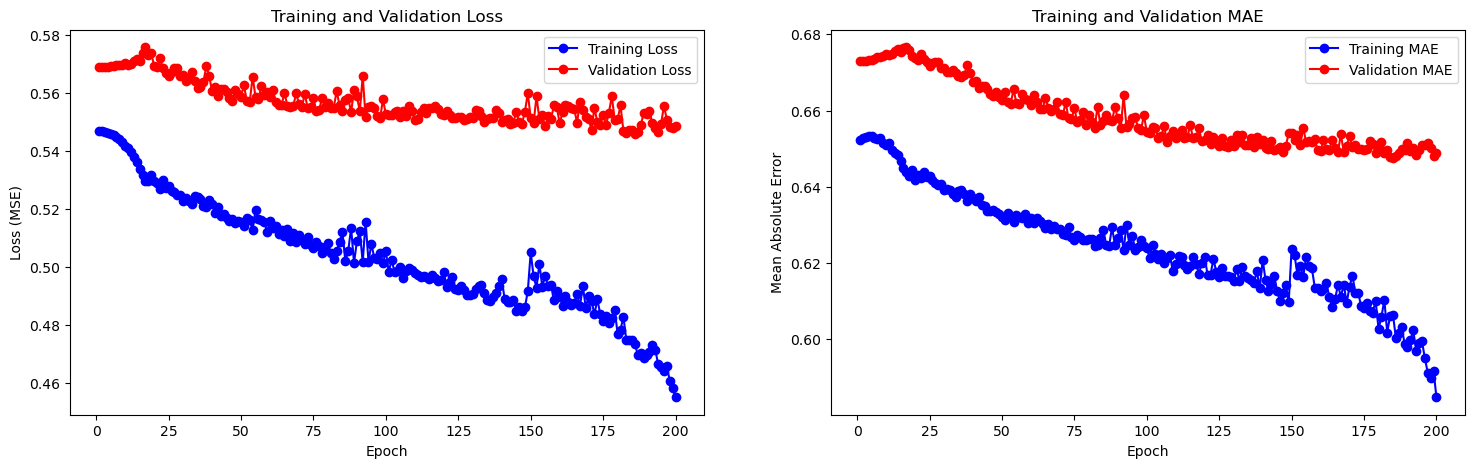
\includegraphics[width=1\linewidth]{updatedLC-hybrid.png}
    \caption {Learning Curves of a 1D-CNN-LSTM Model Over 200 Epochs. The left subplot displays the training and validation MSE loss, while the right subplot illustrates the training and validation MAE.}
    \label{fig:mseless_mae1DCNN-LSTM}
\end{figure}

% Section: Discussion
\section{Discussion}
\label{sec:discussion}    
\noindent This study investigated the prediction of grid cell alignment using advanced machine learning techniques applied to fMRI data. The findings provide critical insights into the neural dynamics of spatial navigation. While traditional tools like GridCAT effectively quantified voxel-wise grid orientations, they relied on generalized linear models (GLMs) that may oversimplify the complex spatial and temporal patterns in the data. By contrast, our application of 1D-CNN and hybrid 1D-CNN-LSTM models revealed the potential and challenges of deep learning for neural data analysis. \\

\subsection{\textbf{GridCAT Analysis}}

The well-defined clustering and orientation in the case of BA as compared to OF might be understood by referencing the original analysis conducted during the data acquisition. When the subject sees a clear boundary, the grid cell alignment is in line with the direction of the boundary wall \cite{he_environmental_2019}. This leads to stronger alignment in the case of BA as compared to OF, irrespective of translation or questioning. This may also be interpreted as a task which is not purely translation, as the barrier provides a cognitive aspect to the task. Studies have looked at the possibility of the grid cells having a role to play in cognitive tasks in addition to pure translation, and the current results from GridCAT suggest that further analysis can follow this hypothesis. This is especially the case for memory dependent cognitive tasks \cite{doeller_evidence_2010}. The flipping of the alignment between translation and questioning provides an interesting counterpoint. It holds in the case of both OF and BA, though the alignment is stronger in the case of BA. 

\subsection{\textbf{1D-CNN Performance Analysis}}
The 1D-CNN model successfully reduced training loss, demonstrating its ability to learn spatial relationships in voxel activation patterns. However, its limited generalization, as evidenced by stagnant validation loss, suggests that the neural data's subtle orientation-dependent features may not be fully captured. The complexity of the neural data, characterized by high-dimensional voxel activations, may contribute to the difficulty in capturing features with strong predictive power across different datasets. The minimal improvement in validation metrics indicates that the neural signatures associated with specific orientation alignments are either too subtle or too variable for the current model architecture to consistently detect. This shows the need for more sophisticated modeling techniques or enhanced data preprocessing to better capture the underlying neural-behavioral relationships and improve the model's predictive accuracy on unseen data.

\subsubsection{Analysis of Predictive Capabilities}

\begin{figure}[htbp]
    \centering
    \begin{minipage}{0.43\textwidth}
        \centering
        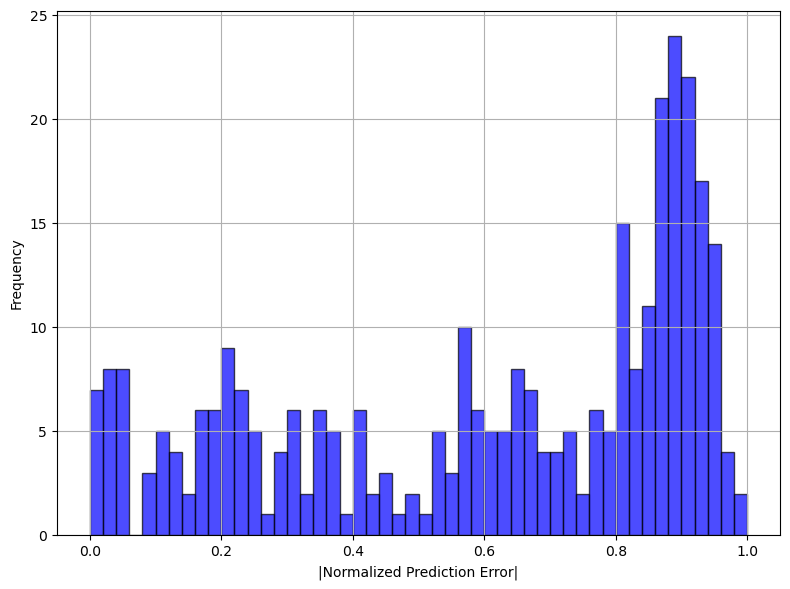
\includegraphics[width=\linewidth]{22.png} % width can be adjusted to your preference
        \caption{Distribution of Absolute Prediction Errors  represent deviations from expected alignment scores, assessing 1D-CNN ability to predict the relationship between stimulus orientations and neural responses.}
        \label{fig:first-image-label}
    \end{minipage}\hfill
    \begin{minipage}{0.53\textwidth}
        \centering
        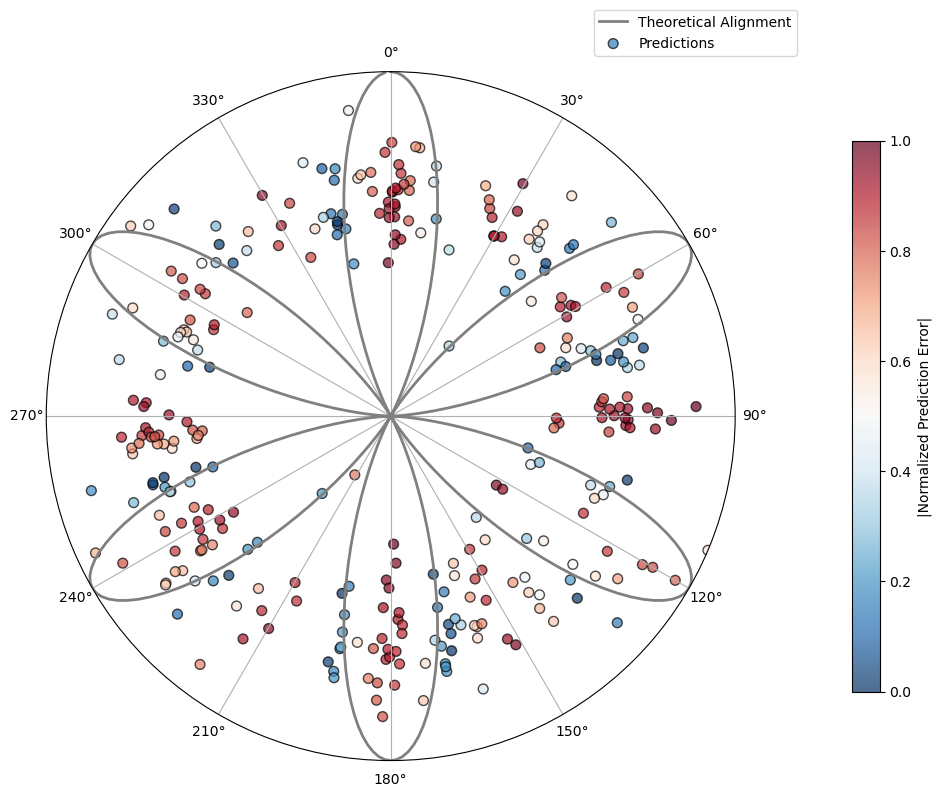
\includegraphics[width=\linewidth]{predictiveerrors1D.png}
        \caption{Prediction Errors Relative to True Orientation Angles and Alignment Scores. This plot maps each true stimulus orientation angle (degrees) to its corresponding prediction error and computed alignment score.}
        \label{fig:1D-CNN histogram}
    \end{minipage}
\end{figure}

\noindent The distribution of normalized absolute prediction errors for the 1D-CNN model shown in Figure \ref{fig:first-image-label}, reveals a predominant concentration of high-error values between 0.8 and 1, indicating that most of the model's predictions significantly deviate from the actual orientation alignments. This right-skewed distribution suggests that the model struggles to accurately map the complex neural activity patterns to their corresponding orientation angles. The high frequency of large errors may be attributed to the intricate and high-dimensional nature of the neural data, which the current model architecture may be insufficiently capturing.

Additionally, Figure \ref{fig:1D-CNN histogram} illustrates a circular plot of the prediction errors of our 1D-CNN model across various true stimulus orientation angles. This analysis aims to determine whether orientations near the preferred alignment angles (0°, 60°, 120°, 180°, 240°, and 300°) are associated with lower prediction errors, thereby indicating stronger predictive power of neural responses at these specific angles. To assess this, we calculated the alignment score for each orientation by determining its minimal angular difference to the nearest preferred angle, as outlined in Equation~\ref{eq:alignment_score},  and categorized the data points into close, moderate, or far proximity groups. Contrary to our hypothesis, orientations closely aligned with preferred angles (within 5-10°) did not exhibit lower prediction errors. The average prediction error for these closely aligned orientations was approximately 0.97, indicating consistently high errors regardless of alignment.

Interestingly, some of the lowest prediction errors occurred at orientations moderately or significantly misaligned. For example, orientations at 344.4654° and 254.8755°, which are roughly 15° and 14.9° away from 0° and 240° respectively, showed exceptionally low prediction errors of 0.007331 and 0.028690. Statistical analysis, including Pearson correlation, revealed no significant linear relationship between angular differences and prediction errors. This indicates that the model’s accuracy is not influenced by how closely an orientation aligns with the preferred angles. These findings suggest that the neural data, irrespective of orientation proximity, may lack distinct features that the model can effectively utilize for accurate predictions. The uniformity in prediction errors across various orientations points to a potential limitation in the model's capacity to capture orientation-specific neural patterns. This highlights the complexity of the neural data and indicates that the current model may require further refinement to enhance its sensitivity to subtle, orientation-dependent neural features.

In conclusion, analysis of 1D-CNN model indicates that orientations near the preferred alignment angles do not confer any advantage in terms of lower prediction errors. The model's performance remains relatively consistent across different orientations, highlighting a potential limitation in its ability to capture orientation-specific neural patterns. This lack of association highlights the complexity of the neural data and suggests that the current model may require further refinement to enhance its sensitivity to subtle, orientation-dependent neural features. 


\subsection{\textbf{1D-CNN-LSTM Performance Analysis}}
Interestingly, the 1D-CNN-LSTM model showed modest improvements, with reduced prediction errors in alignment scores associated with preferred orientations, highlighting the significance of incorporating temporal dependencies. Nevertheless, both models struggled to reliably predict alignment scores for non-preferred orientations, potentially reflecting the high dimensionality and variability of the BOLD signals.\\

\subsubsection{Analysis of Predictive Capabilities}

Comparative analysis of the 1D-CNN and 1D-CNN-LSTM models reveal notable differences in their predictive capabilities. As depicted in Figure \ref{fig:APErrors CNNLSTM}, the 1D-CNN-LSTM model demonstrates a more favorable distribution of prediction errors, with the majority ranging between 0\% to 50\%. In contrast, the 1D-CNN model exhibits a significant portion of errors concentrated in the 80\% to 100\% range. Although the improvement in predictive accuracy is modest, integrating the LSTM layer into the 1D-CNN-LSTM model enhances its ability to process temporal information in short data sequences. This capability allows the model to better capture subtle temporal dependencies in neural responses, leading to a reduction in prediction errors compared to the 1D-CNN model.\\

\begin{figure}[htbp]
    \centering
    \begin{minipage}{0.43\textwidth}
        \centering
        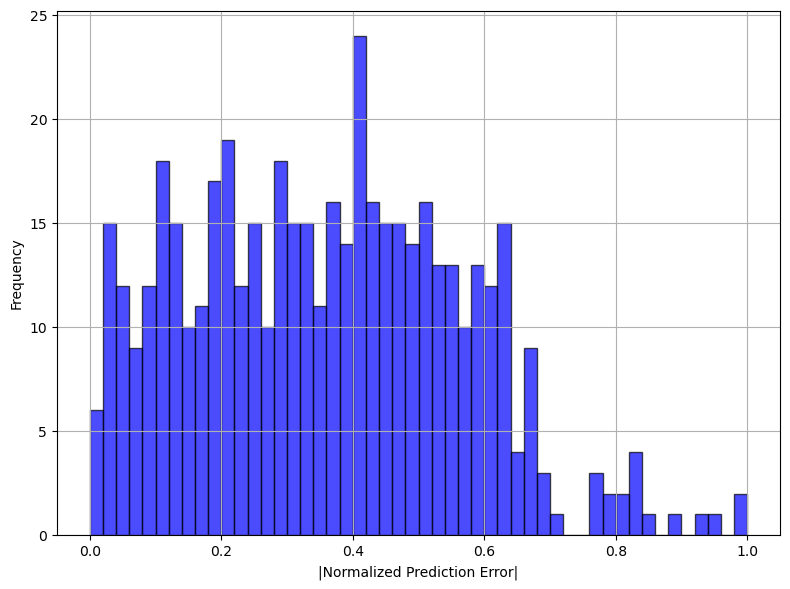
\includegraphics[width=\linewidth]{lstmhistogram.png} 
        \caption{Distribution of Absolute Prediction Errors  represent deviations from expected alignment scores, assessing 1D-CNN-LSTM ability to predict the relationship between stimulus orientations and neural responses.}
        \label{fig:APErrors CNNLSTM}
    \end{minipage}\hfill
    \begin{minipage}{0.53\textwidth}
        \centering
        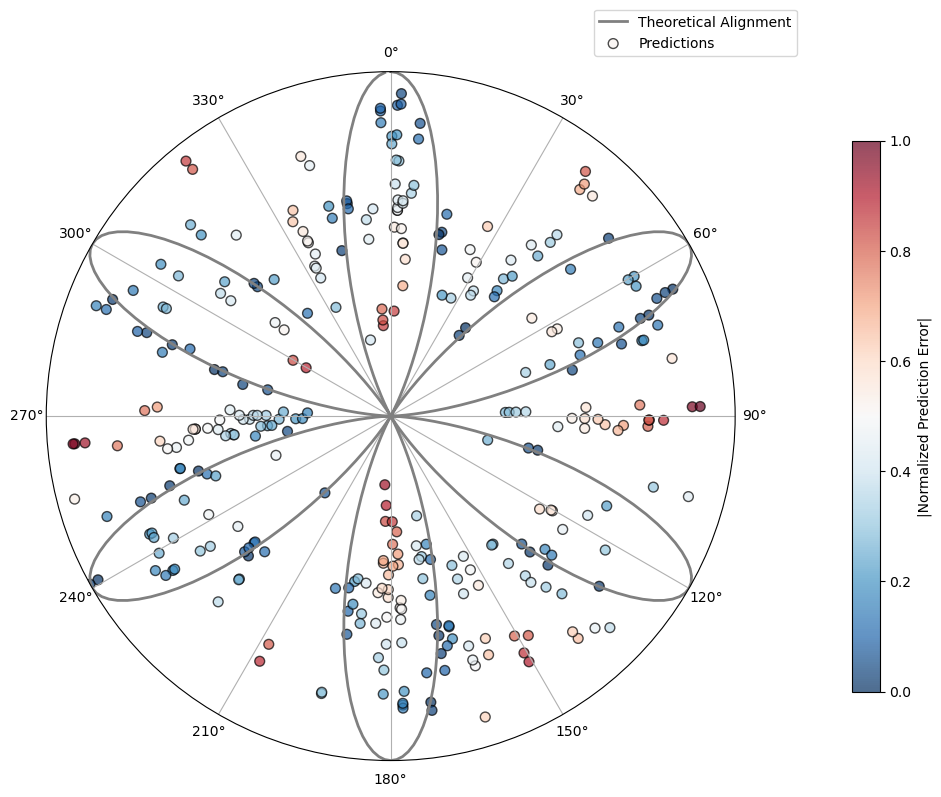
\includegraphics[width=\linewidth] {1d-cnn-lstm-model.png}
        \caption{Prediction Errors Relative to True Orientation Angles and Alignment Scores. This plot maps each true stimulus orientation angle (degrees) to its corresponding prediction error and computed alignment score.}
        \label{fig:PredictHybrid}
    \end{minipage}
\end{figure}

\noindent Figure \ref{fig:PredictHybrid} displays the predicted alignment scores plotted on a circular graph corresponding to the orientation angles of the stimuli. In this visualization, angle of each point represents the stimulus orientation, the radius corresponds to the predicted alignment score (reflecting the strength of the BOLD signal), and the color indicates the magnitude of the prediction error. This circular plot allows us to assess how effectively the model captures the inherent periodicity of neural responses to different stimulus orientations.

The model appears to perform reasonably well in predicting orientation alignment at the preferred orientations around 0°, 60°, 120°, 180°, 240°, and 300°, where neurons are most responsive. Points located near the circumference of the circle, representing higher predicted alignment scores and stronger BOLD intensities, generally show lower absolute prediction errors between 0 and 0.5. In contrast, points closer to the center, indicating lower predicted alignment scores and weaker BOLD responses, tend to exhibit higher absolute prediction errors. These observations suggest that the model effectively associates higher BOLD intensities with preferred orientations, successfully capturing strong neural activations. However, the higher prediction errors for orientations associated with lower BOLD signals indicate a potential bias in the model. It seems less accurate in predicting alignment scores for less pronounced neural responses, possibly due to challenges in modeling weaker signals. This limitation highlights the model's reduced sensitivity to subtle neural responses associated with non-preferred orientations.

While 1D-CNN-LSTM demonstrates the ability to capture key patterns in neural data, particularly for strong activations at preferred orientations, there is room for improvement in accurately modeling weaker neural responses. Addressing this bias could enhance the model's predictive accuracy across the full range of stimulus orientations.


\subsection{\textbf{Model Limitations, data constraints and potential sources of error}}
Our results align with previous literature on the challenges of predicting neural responses to spatial stimuli. For example, prior studies using fMRI data also reported difficulties in capturing grid cell alignment, particularly in variable behavioral contexts. Unlike earlier approaches limited by linear assumptions, our neural networks aimed to uncover complex patterns, albeit with limited success in generalization. This underscores the need for hybrid models and enhanced preprocessing techniques to disentangle the intricate neural-behavioral relationships.

Limitations of the study include a small dataset, which constrained the models' ability to generalize and increased the risk of overfitting. Additionally, potential noise in the BOLD signal and preprocessing steps, such as masking and temporal alignment, may have contributed to prediction errors. Future work should focus on expanding the dataset, optimizing model architectures, and incorporating regularization techniques to improve sensitivity to subtle neural patterns.

% Section: Conclusion
\section{Conclusion}
\label{sec:conclusion}

\noindent This study demonstrated the application of machine learning techniques, including 1D-CNN and hybrid CNN-LSTM models, to predict grid cell alignment from fMRI data. While these models showed promise in capturing spatial and temporal features, their performance was hindered by limited generalization to unseen data. The findings highlight the potential of deep learning to analyze complex biological data, such as voxel-based neural responses, while underscoring the challenges posed by high-dimensional and variable signals.

The results emphasize the need for advanced preprocessing and hybrid modeling approaches to improve accuracy and robustness. Furthermore, the study reinforces the importance of grid cell-like activity as a cornerstone of spatial navigation research and paves the way for future applications of machine learning to probe neural dynamics. Expanding the dataset and refining the architectures could uncover deeper insights into the relationship between neural activity and behavioral stimuli.


% References
\printbibliography[heading=bibintoc, title={References}]

\end{document}
